\newpage
\section{SYSTEM DESIGN}

\subsection{System Overview}
The system uses initially predicts the personality of the user with the help of their social media account(facebook). Thus initially a classifier is to be trained to classify the personality of the user on the basis of their status update. Afterwards, the predicted personality of the user is to be used as one the metrics for the similar user computation in collaborative filtering and the effect of the personality on the collaborative filtering engine was observed.

\subsection{System Architecture}
The give figure below is the architectural diagram of the project showing the process that are involved during the development of the project.

\begin{figure}[!ht]
\centering
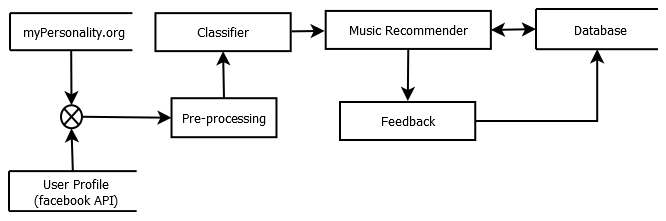
\includegraphics[width = 16 cm]{fig/new/system.png}
\caption{Block Diagram of the System}
\label{fig:project}
\end{figure}

\begin{itemize}
	\item Pre-processing Unit/Data Preprocessor: This subsystem is responsible for the conversion of the status update of the user from the dataset \cite{dataset} as well user logged in via API \cite{api} into vector representation via the use of bag of word and tf-idf model.\\
It is responsible for:
		\begin{enumerate}
			\item Lower casing the status update.
			\item Tokenization
			\item Filtering stop words
			\item Filtering parts of speech
			\item Stemming
			\item Conversion of textual data to vector representation(numerical form)
		\end{enumerate}
The following figure depicts tasks performed within preprocessor unit within the system:
\begin{figure}[!ht]
\centering
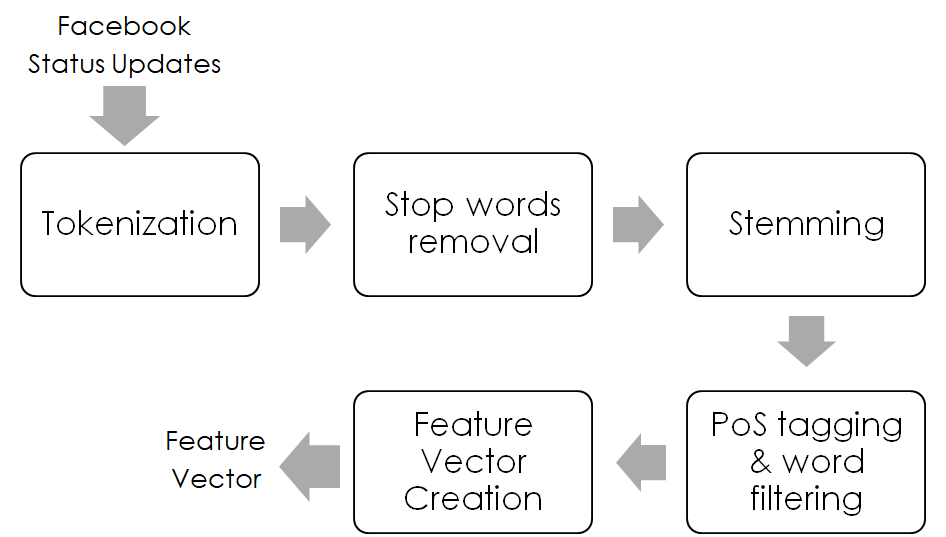
\includegraphics[width = 16 cm]{fig/preprocessing.png}
\caption{Tasks performed by preprocessor unit within the system}
\label{fig:project}
\end{figure}
	\item Classifier: After the vector representation of the status update,this subsystem is responsible for personality prediction. Classifier are trained by the admin in the system using the dataset \cite{dataset} in order to predict a personality. In the project there are two classifier model used for the personality classification.\\
They are:
\begin{enumerate}
	\item Naive Bayes Classifier
	\item Logistic Regression
\end{enumerate}
The following figure depicts tasks performed by classifier unit within the system:
\newpage
\begin{figure}[!h]
\centering
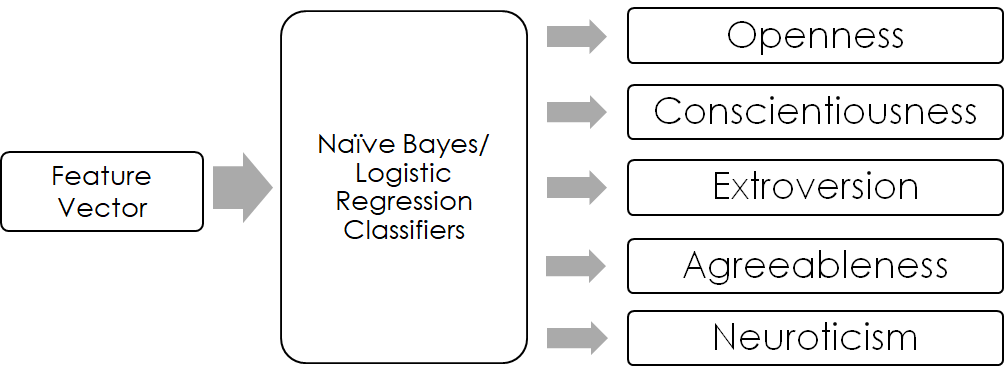
\includegraphics[width = 16 cm]{fig/classification_block_diagram.png}
\caption{Tasks performed by classifier unit within the system}
\label{fig:project}
\end{figure}
\item Music Recommender System: The system comprises of the eight models for the recommendation of the music to the user.\\
They are:
\begin{enumerate}
	\item Global Baseline Approach
	\item User to User collaborative filtering with rating matrix
	\item User to User collaborative filtering with personality matrix
	\item User to User collaborative filtering with weighted average of rating and personality matrix
	\item Combination of global baseline and CF with rating matrix
	\item Combination of global baseline and CF with personality matrix
	\item Combination of global baseline and CF with weighted average of rating and personality matrix
	\item Matrix Factorization
\end{enumerate}
The following figure summarizes tasks performed by recommender unit within the system:
\newpage
\begin{figure}[!ht]
\centering
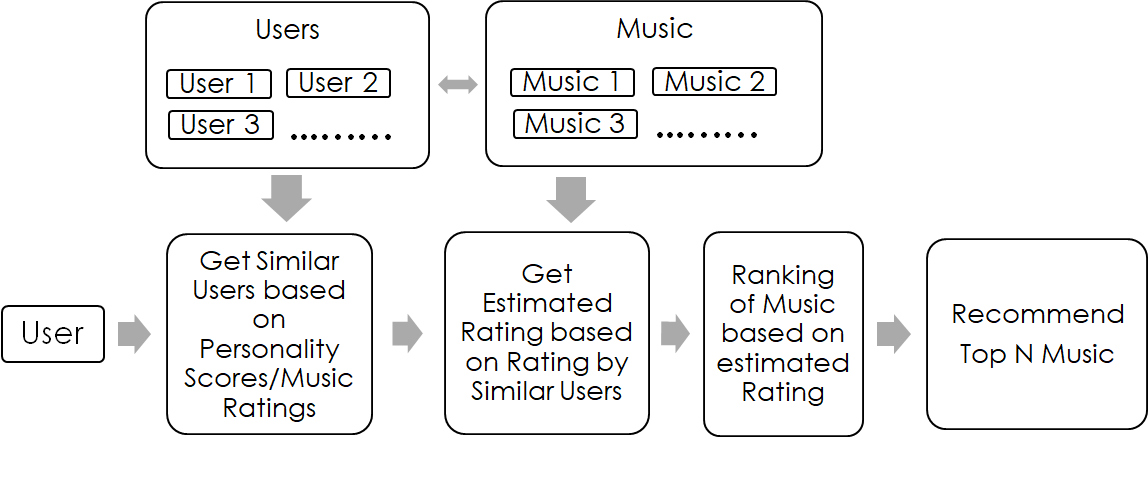
\includegraphics[width = 16 cm]{fig/recommendation_block_diagram.png}
\caption{Tasks performed by recommedation unit within the system}
\label{fig:project}
\end{figure}
The following figure depicts various recommendation models used within the system:
\begin{figure}[!ht]
\centering
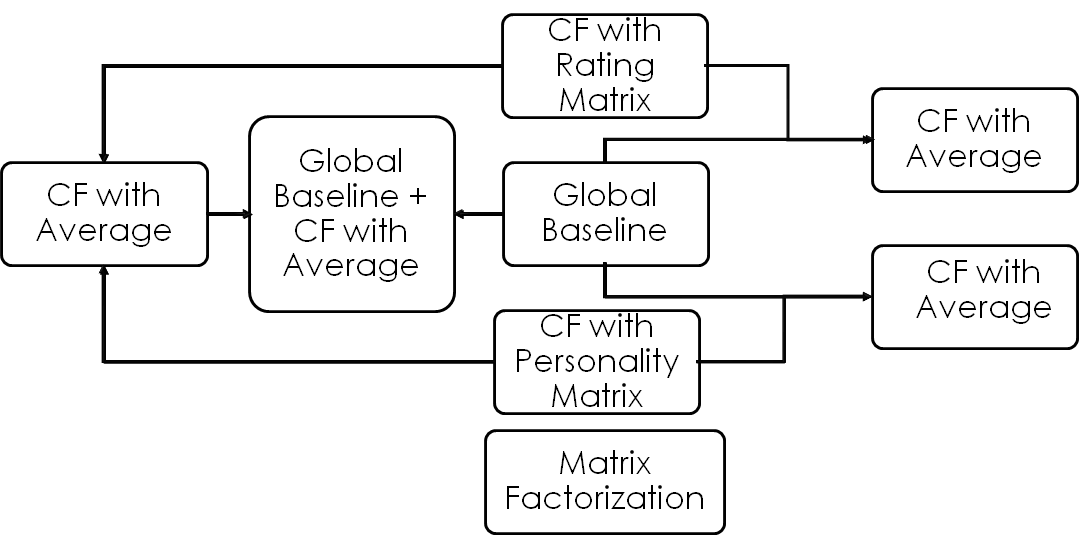
\includegraphics[width = 16 cm]{fig/recommendation_models.png}
\caption{Recommedation models used within the system}
\label{fig:project}
\end{figure}
\item Storage Unit/Database: It is responsible for storing of user data, music data, user-music-rating data and user-music-recommendation data made by the recommender system as well as providing recommendation based on user-feedbback. SQLite database is used as the storage unit for the project.
\end{itemize}

\newpage
\subsection{Use Case Diagram}
A use case diagram represents user's interaction with the system that shows the relationship between the user and the different use cases in which the user is involved. A use case diagram can identify different types of users of a system, different use cases as well. A use-case diagram provides higher-level view of the system. Use case diagrams are the blueprints for the system. The use cases are shown as ovals, actors as stick people (even if they are machines), with lines (known as associations) connecting use cases to the actors who are involved with them. A box around the use cases emphasizes the boundary between the system (defined by the use cases) and the actors who are outside of the system. In our case, actor 'user' can log in to the system, allow system to access his profile information and view output or result from the system.% Similar is the case for 'system' and 'sysadmin'. 
\\
Use case diagram of the system depicting the actors and their interaction to the system is given in the figure below:
\begin{figure}[!ht]
\centering
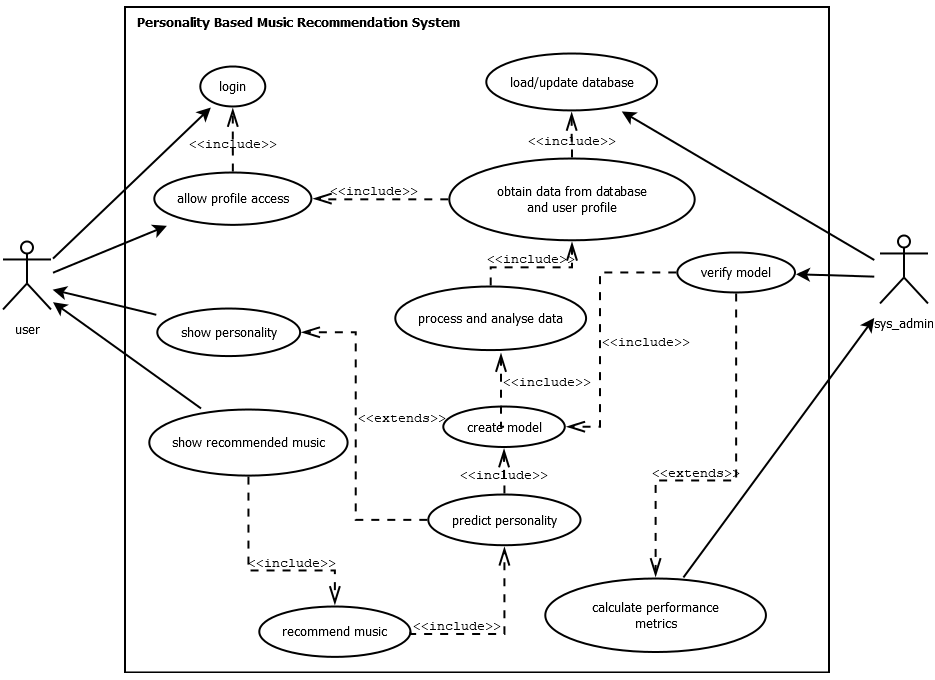
\includegraphics[width = 16 cm]{fig/new/usecase.png}
\caption{Use Case Diagram of the System}
\label{fig:usecase}
\end{figure}

From the above diagram, it is clear that the system consists of two actors.They are:
\begin{itemize}
\item User: They are the ones who will be using the system directly. The users will be able to do the actions like login, viewing recommendation and listening to a music.
\item Admin: Admin is directly responsible for training a classifier subsystem and recommender subsystem, creation of model for the storage engine and verification of all of these subsystem.
\\
System is composed of ui, classifier, music recommender and storage unit.Classifer within the system is responsible for the classification of the personality of the user and update of the database. Recommender is responsible for the recommendation of the music to the user and also update of the database.Storage unit is responsible for the creation of the data base model and storage of system data and ui is responsible for providing user with login access, profile access and displaying user a personality and recommendation of music.
\end{itemize}

\newpage
\subsection{ER Diagram}

An Entity-Relationship model describes inter-related things of interest in a specific domain of knowledge. In software development, ER model has become an abstract data model that defines a data/information structure that can be implemented in a database, typically a relational database. In our database, we have separate tables for user, music, recommendation and session. Each table has several attributes that best describe the table. To get required information, say we need to print details of particular user, we need to access database and more than one tables to retrieve data. We need certain relationship between each tables in our database and a common attribute to map tuples of one table to another. ER Diagram provides visual reference to complete database at one glance. We can develop database looking at the ER Diagram and later use it as reference for further improvement. 
\\
The  ER diagram depicting the entities used in the system and relationship between them is given below:
\begin{figure}[!ht]
\centering
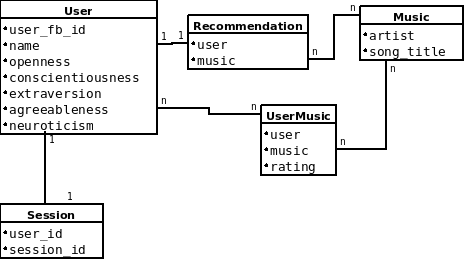
\includegraphics[width = 10 cm]{fig/er.png}
\caption{ER diagram of the System}
\label{fig:er}
\end{figure}
The entities in the system are:
\begin{enumerate}
	\item Session: It consists of attributes: session id and user id and has one to one relationship with user.
	\item Music: It consists of attributes: artist and song title and also has  many to many relationship with the user-music and recommendation.
	\item User: It consists of attributes user id, name and personality traits attributes and has  many to  many relationship with user-music and one to one with the session with session and recommendation.
	\item Recommendation: It consists of attributes user and music and has one to one relationship with user while many to many relationship with music.

	\item User-Music: It consists of attributes user, music and rating and many to many relationship with user and music.
\end{enumerate}
System is implemented within the Django framework that provides a abstraction to the relationship within the database hence we can directly implement those relationship within the database such as one-to-one, one-to-many and many-to-many.
\subsection{Activity Diagram}
Activity Diagram describes the dynamic aspects of the system. It diagram shows user oriented view of system operation. We have made activity diagram using swim-lanes. A swim lane is a visual element that distinguishes job sharing and responsibilities for sub-processes. In our system's activity diagram, we have three swim-lanes and we have separated job/responsibilities accordingly. Each step is continuation of previous step. Decision is taken wherever necessary and fork and join is used to divide or attach work flow. The objective of making activity diagram is similar to objectives of other UML Diagrams. Only difference is that it is used to show message flow between activities.
\newpage
\begin{figure}[!ht]
\centering
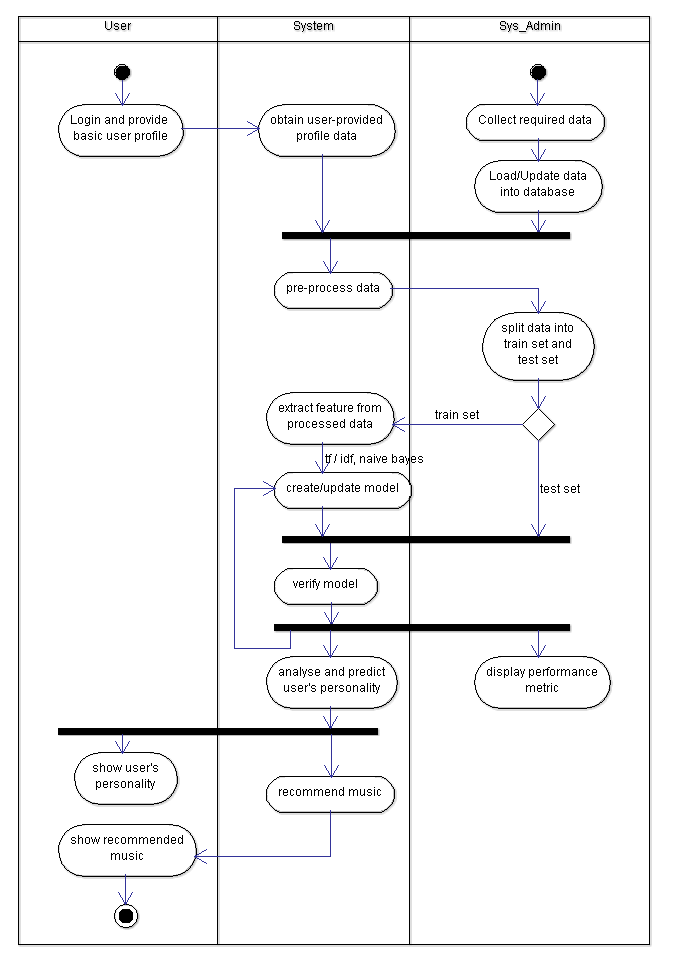
\includegraphics[width = 12 cm]{fig/new/activity.png}
\caption{Activity Diagram of the System}
\label{fig:activity}
\end{figure}

The diagram above shows the activity digram of the system. It depicts how the user, admin and system interacts with each other. Initially user login into the system providing the basic user profile information. Afterwards, the status of the new/old user is used to predict the personality with classifier. Then music is recommended to user. Besides, the user can also view his personality.

\newpage
\subsection{Context Diagram}

A system context diagram (SCD) in engineering is a diagram that defines the boundary between the system, or part of a system, and its environment, showing the entities that interact with it. This diagram is a high level view of a system. It is similar to a block diagram. In our system context diagram, there are two entities namely, user and sysadmin and a process (which is the system we developed as our project). This diagram shows the input and output for each of the entity as well as the process.
\begin{figure}[!ht]

\centering
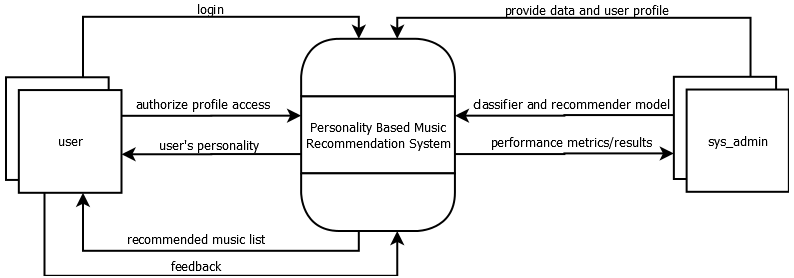
\includegraphics[width = 16 cm]{fig/new/dfd0.png}
\caption{Context Diagram of the System}
\label{fig:dfd0}
\end{figure}
\subsection{Data Flow Diagram}
A data flow diagram (DFD) is a graphical representation of the "flow" of data through an information system, modelling its process aspects. A DFD shows what kind of information will be input to and output from the system, how the data will advance through the system, and where the data will be stored. However, it does not show information about process timing or whether processes will operate in sequence or in parallel Being a UML diagram, DFD presents both control and data flows as a unified model. Given diagram is the level-0 DFD that shows internal distinct process of our system. There are four processes and a datastore which stores all data, intermediate outcomes and results. Two entities, user and sysadmin, take part in flow of data to/from these process. Each arrow head in the data flow diagram shows the direction of the data/information flow and label provide type of data/information that flows through.
The figure given below is the data flow diagram of the project showing the flow of data within the system.


\begin{figure}[!ht]
\centering
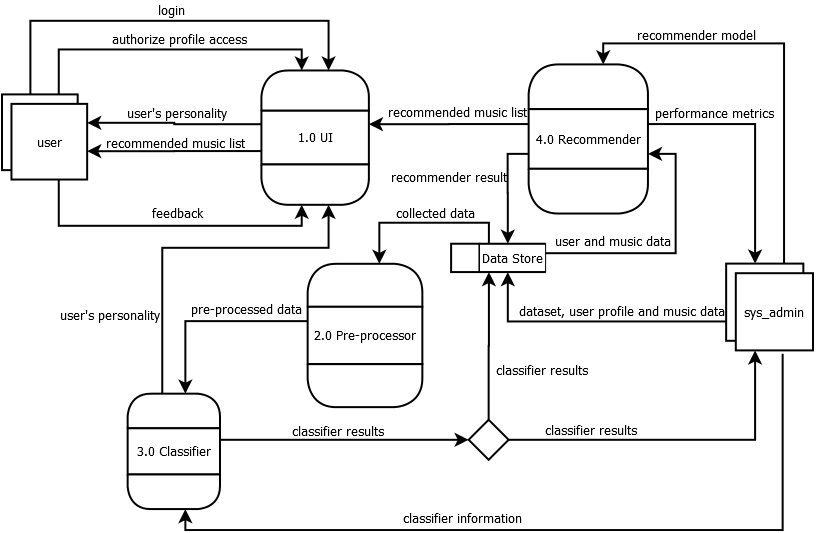
\includegraphics[width = 16 cm]{fig/new/dfd.png}
\caption{Data Flow Diagram of the System: level-0}
\label{fig:dfd}
\end{figure}

It is the level-0 dfd, with the two entities User and Admin. User is responsible for log in, view personality and view recommended music, all of which takes data from the user and recommendation store, to provide a data to the user. Besides admin is responsible for creating and altering models(classifier,recommender,database) all of which are reflected within the user and recommendation store.

\subsection{Front End of the System(User Interface)}
User Interface is one of the major part of the system. It is where a user will login through their Facebook id in order to experience the personalized based music listening. User is able to able to view his/her recommended music as well as personality via the website and also view the detailed description about the personality traits. Personality classification and music recommendation are all performed in the backend of the system.

% Following are the snapshots of our system UI:
% \begin{figure}[!ht]
% \centering
% 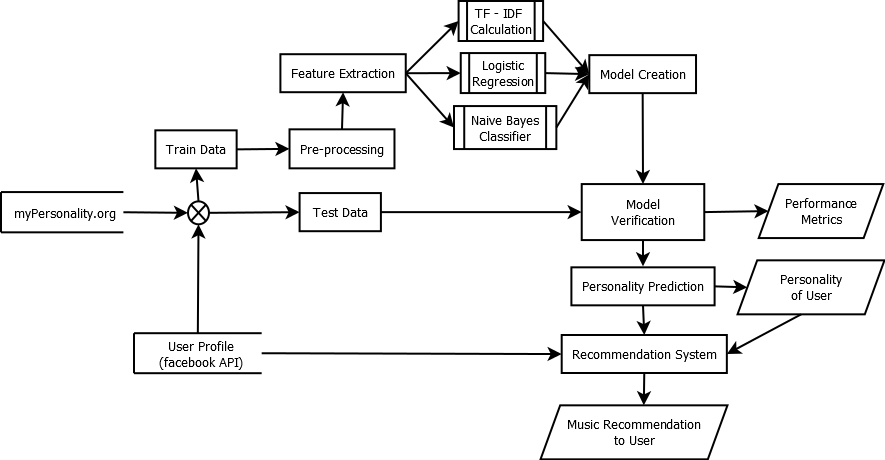
\includegraphics[width = 16 cm]{fig/System.png}
% \caption{Front of the System}
% \label{fig:front}
% \end{figure}

% \newpage
\subsection{Back End of the System}
After the user login through Facebook, the user post are extracted through Graph API. The data obtained goes through the preprocessor where it's performs various NLP techniques such as tokenization, POS tagging at the end of which feature vector is given as output by this subsystem. Thus created vector is passed through the classifier, that classifies the personality of the user, which is then stored in the database and is also fed into user-to-user collaborative filtering engine to determine the similar user and recommend the music to the user.Besides there are also other recommendation model, one with the least RMSE value is used for the recommendation of the music. Thus obtained result is sent back to the front end and is displayed to the user. Then the user can view recommended music and his/her personality traits too.
